\documentclass{jlreq}

\usepackage{fontspec}
\usepackage{unicode-math}
\setmainfont{Latin Modern Roman}
\setmathfont{Latin Modern Math}
\usepackage{pgfplots}
\pgfplotsset{compat=1.18}
\usepgfplotslibrary{statistics}

\begin{document}
qq
kk
これはテストです。English and math: \( \frac{\sin r}{r} \)
ガウス関数の導出をします。
\begin{align*}
    f(x)                               & = \frac{1}{\sqrt{2\pi}} e^{-\frac{x^2}{2}}                               \\
    \int_{-\infty}^{\infty} f(x) \, dx & = \int_{-\infty}^{\infty} \frac{1}{\sqrt{2\pi}} e^{-\frac{x^2}{2}} \, dx \\
                                       & = \frac{1}{\sqrt{2\pi}} \int_{-\infty}^{\infty} e^{-\frac{x^2}{2}} \, dx \\
                                       & = \frac{1}{\sqrt{2\pi}} \cdot \sqrt{2\pi}                                \\
                                       & = 1
\end{align*}
複素数の積分を考えますss
\begin{align*}
    \int_{-\infty}^{\infty} e^{ix} \, dx & = \lim_{R \to \infty} \int_{-R}^{R} e^{ix} \, dx                                               \\
                                         & = \lim_{R \to \infty} \left[ \frac{e^{ix}}{i} \right]_{-R}^{R}                                 \\
                                         & = \lim_{R \to \infty} \left( \frac{e^{iR}}{i} - \frac{e^{-iR}}{i} \right)                      \\
                                         & = \lim_{R \to \infty} \left( \frac{\cos R + i \sin R}{i} - \frac{\cos R - i \sin R}{i} \right) \\
\end{align*}
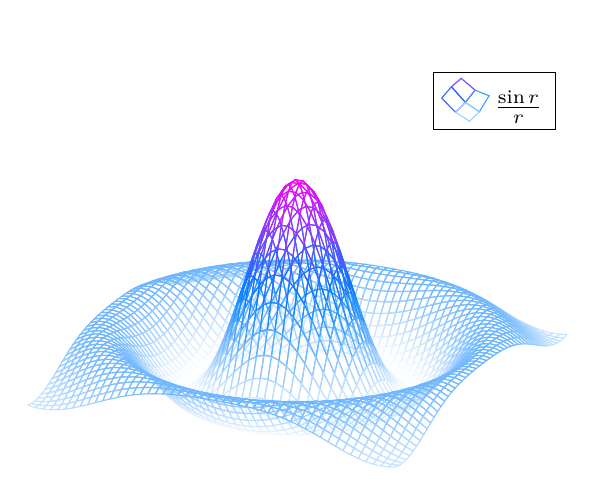
\begin{tikzpicture}
    \begin{axis}[
            title=グラフタイトル,
            colormap/cool,
            hide axis,
        ]
        \addplot3[
            mesh,
            samples=50,
            domain=-8:8,
        ]
        {sin(deg(sqrt(x^2+y^2)))/sqrt(x^2+y^2)};
        \addlegendentry{$\frac{\sin r}{r}$}
    \end{axis}
\end{tikzpicture}

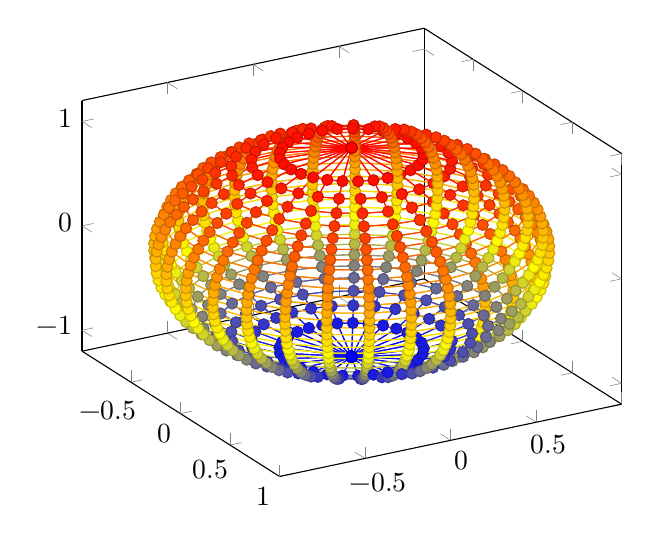
\begin{tikzpicture}
    \begin{axis}[view={60}{30}]
        \addplot3 [
            only marks,
            mesh,z buffer=sort,
            scatter,scatter src=z,
            samples=30,domain=-1:1,y domain=0:2*pi,
        ] (
        {sqrt(1-x^2) * cos(deg(y))},
        {sqrt( 1-x^2 ) * sin(deg(y))},
        x
        );
    \end{axis}
\end{tikzpicture}

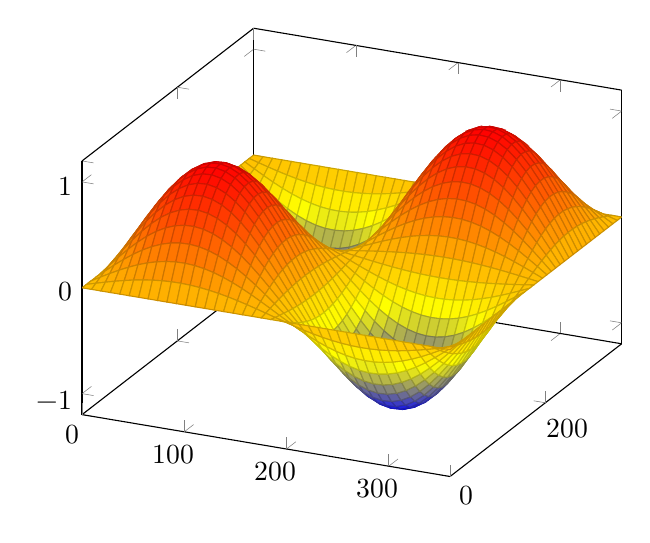
\begin{tikzpicture}
    \begin{axis}
        \addplot3 [
            surf,
            domain=0:360,
            samples=40,
        ] {sin(x)*sin(y)};
    \end{axis}
\end{tikzpicture}




\end{document}
